% !TeX root = ../main.tex
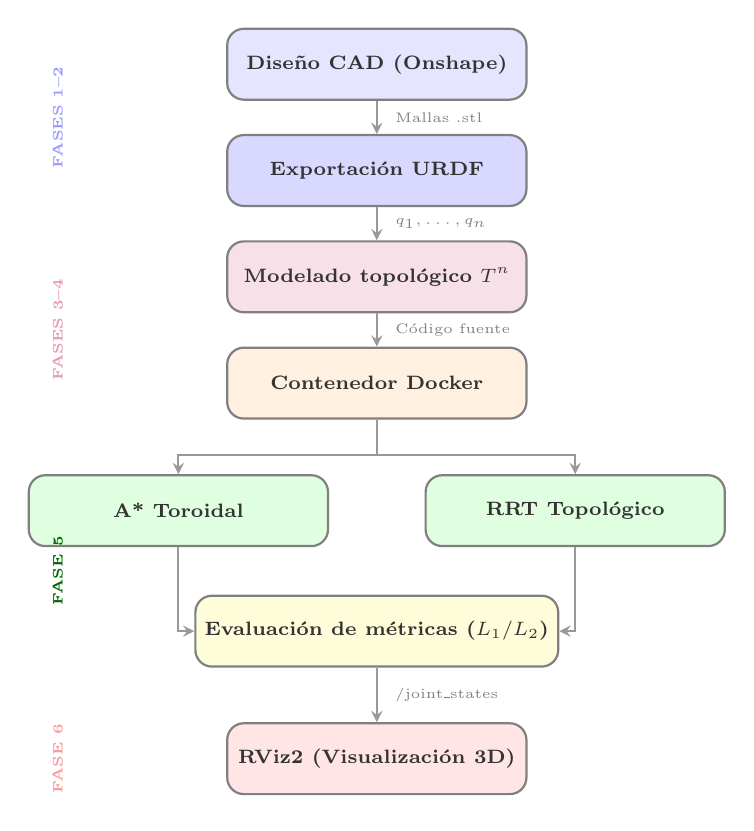
\begin{tikzpicture}[>=stealth, scale=0.9, every node/.style={font=\small},
    % Estilos
    phase/.style={
        draw=black!50, thick, rounded corners=6pt,
        fill=#1, minimum width=3.8cm, minimum height=0.9cm,
        font=\scriptsize\bfseries, align=center, text=black!80
    },
    conn/.style={
        ->, thick, black!40
    },
    lbl/.style={
        font=\tiny, text=black!50
    }
]

% =============================================
% COLUMNA PRINCIPAL (flujo vertical)
% =============================================

% Fase 1
\node[phase=blue!10] (cad) at (0, 0) {Diseño CAD (Onshape)};

% Fase 2
\node[phase=blue!15] (urdf) at (0, -1.5) {Exportación URDF};
\draw[conn] (cad) -- (urdf) node[lbl, midway, right=3pt] {Mallas .stl};

% Fase 3
\node[phase=purple!12] (topo) at (0, -3.0) {Modelado topológico $T^n$};
\draw[conn] (urdf) -- (topo) node[lbl, midway, right=3pt] {$q_1, \dots, q_n$};

% Fase 4
\node[phase=orange!12] (docker) at (0, -4.5) {Contenedor Docker};
\draw[conn] (topo) -- (docker) node[lbl, midway, right=3pt] {Código fuente};

% =============================================
% BIFURCACIÓN: Algoritmos (paralelo)
% =============================================
\node[phase=green!12] (astar) at (-2.8, -6.3) {A* Toroidal};
\node[phase=green!12] (rrt)   at ( 2.8, -6.3) {RRT Topológico};

\draw[conn] (docker.south) -- ++(0,-0.5) -| (astar.north);
\draw[conn] (docker.south) -- ++(0,-0.5) -| (rrt.north);

% =============================================
% CONVERGENCIA: Evaluación
% =============================================
\node[phase=yellow!15] (eval) at (0, -8.0) {Evaluación de métricas ($L_1 / L_2$)};
\draw[conn] (astar.south) |- (eval.west);
\draw[conn] (rrt.south)   |- (eval.east);

% =============================================
% SALIDA FINAL
% =============================================
\node[phase=red!10] (rviz) at (0, -9.8) {RViz2 (Visualización 3D)};

\draw[conn] (eval.south) -- (rviz.north)
    node[lbl, midway, right=3pt] {/joint\_states};

% =============================================
% ETIQUETAS DE FASE (barra lateral izquierda)
% =============================================
\node[rotate=90, font=\tiny\bfseries, blue!40]   at (-4.5, -0.75) {FASES 1--2};
\node[rotate=90, font=\tiny\bfseries, purple!40] at (-4.5, -3.75) {FASES 3--4};
\node[rotate=90, font=\tiny\bfseries, green!40!black]  at (-4.5, -7.15) {FASE 5};
\node[rotate=90, font=\tiny\bfseries, red!40]    at (-4.5, -9.8)  {FASE 6};

\end{tikzpicture}

